\katzper{This section should probably be entirely rewriten to use \cref{thm:segments-theorem}.}

Following the notation from the previous sections, we write $f \equiv g$ if the equality of $f$ and $g$ can be proved using rules.

\begin{theorem}\label{thm:simple-functions-completeness}
    For every pair of simple functions $f,g : A \to \Gamma^*$, if $f = g$, then $f \equiv g$.
\end{theorem}

The rest of this section is devoted to proving \cref{thm:simple-functions-completeness}. We proceed by a nested induction. The outer induction is on the rank of type $A$ \katzpermargin{define the rank of type}. Once the type is fixed, we write
\begin{gather*}
    f = \delta_0 \cdot f_1 \cdot \delta_1 \cdots \delta_{n-1} \cdot f_n \cdot \delta_n \\
    g = \gamma_0 \cdot g_1 \cdot \gamma_1 \cdots \gamma_{m-1} \cdot g_m \cdot \gamma_m,
\end{gather*}
where $f_1, \dots, f_n, g_1, \dots, g_m$ are bihomomorphisms ($\leftarrow$ or $\rightarrow$) on one of the root lists, and $\delta_0, \dots, \delta_n, \gamma_0, \dots, \gamma_m$ are functions on $(\first{A}, \last{A})$. Then, the inner induction is on $n+m$.

We assume that no $f_i$, $g_j$ is equal to $\varepsilon$, otherwise we can eliminate it.

We start with some simple cases. If $A = 1$, then the only possible functions are constant, so we actually need a rule for them? \katzpermargin{how do we formally resolve constant functions?} If $n = 0$ or $m = 0$, then it must hold that either $n = m = 0$, in which case we reduce to a simpler type, or there is some $f_i = \varepsilon$ (or $g_j = \varepsilon$), which we can eliminate.

First, we show that only three cases can occur: (1) $n = m = 1$, (2) all $f_1, \dots, f_n,g_1, \dots, g_m$ are unary, or (3) we can find a proper good interface and split reasoning into two separate parts.

For $i \in [n]$, by $\sfpref{f}{i}$ we denote the function $f_1 \cdot \delta_1 \cdots \delta_{i-1} \cdot f_i$. Analogously we define $\sfpref{g}{j}$ for $j \in [m]$.

\begin{lemma}\label{lemma:the-only-three-cases-for-simple-functions}
    Suppose that $f = g$ and $n, m \geq 1$. Then at least one of the following must hold:
    \begin{enumerate}
        \item $n = m = 1$,
        \item there exists prime $u \in \Gamma^*$ such that $\sfpref{f}{n}$ and $\sfpref{g}{m}$ are $u$-unary, or
        \item there exist $i \in [n], j \in [m]$, such that $1 \leq i + j < n+m$ and $\rint{\delta_0 \cdot \sfpref{f}{i}}{\gamma_0 \cdot \sfpref{g}{j}}$ is good.
    \end{enumerate}
\end{lemma}

Before we prove \cref{lemma:the-only-three-cases-for-simple-functions}, we show progress in all of the tree cases.

\begin{claim}\label{claim:progress_for_unary}
    If $f = g$ and there exists prime $u \in \Gamma^*$ such that $\sfpref{f}{n}$ and $\sfpref{g}{m}$ are $u$-unary, then $f \equiv g$.
\end{claim}

\begin{proof}
    \katzper{TODO}
\end{proof}


\begin{lemma}\label{lem:bihom-equality-is-provable}
    If $\bihom{to, f} = \bihom{to, g}$ then $\bihom{to, f} \equiv \bihom{to, g}$
\end{lemma}
\begin{proof}
    We will find a simple function with group output $h$, with the following properties:
    \begin{itemize}
        \item  ${h|}_{A_1} \equiv \epsilon$
        \item  $h(x)g(x, y) \equiv f(x, y)h(y)$
    \end{itemize}

    The result will follow from axiom \cref{rule:bihom-rotation}.

    Let $a_0$ be a fixed element of $A_1$.
    Define $h(x) := \rint{g(a_0, x)}{f(a_0, x)}$.

    $h(A_1) = \epsilon$ because then for any $[a_0, a]$ forms a valid input to $\bihom{to, f}$ and $\bihom{to, g}$, so they agree on it, and the interface is empty.

    Note that with this definition items (i) and (ii) are equivalent to \dots \kacpermargin{Explain that those two facts are about concatenations of (subgroup) simple functions, so they are provable by induction.}

    Since $f, g$ are used under a homomorphism it is natural to apply them to tuples longer than a pair. Below I write $f(x, y, z)$ to denote $f(x, y)f(y, z)$ and similarily for four inputs.

    Since $f(a_0, y, a_0) = g(a_0, y, a_0)$  and $f(a_0, x, y, a_0) = g(a_0, x, y, a_0)$ and it is on a simpler type, we have:


    from them we can deduce

    \begin{align}
        f(a_0, y, a_0)           & \equiv g(a_0, y, a_0)\notag                               \\
        f(y, a_0)\inv{g(y, a_0)} & \equiv \inv{f(a_0, y)}g(a_0, y) \label{eq:3-element-list}
    \end{align}

    \begin{align}
        f(a_0, x, y, a_0)        & \equiv g(a_0, x, y, a_0)\notag                                           \\
        f(y, a_0)\inv{g(y, a_0)} & \equiv \inv{(f(a_0, x)f(x, y))}g(a_0, x)g(x, y)\label{eq:4-element-list}
    \end{align}

    We can now deduce $h(x) \cdot g(x, y) \equiv f(x, y) \cdot h(y)$, which finishes the proof.

    \begin{align*}
        f(y, a_0)\inv{g(y, a_0)} \equiv f(y, a_0)\inv{g(y, a_0)} \tag{idendity}                                    \\
        f(y, a_0)\inv{g(y, a_0)} \equiv \inv{(f(a_0, y)}g(a_0, y)) \tag{by \cref{eq:3-element-list}}               \\
        \inv{(f(a_0, x)f(x, y))}g(a_0, x)g(x, y) \equiv \inv{f(a_0, y)}g(a_0, y) \tag{by \cref{eq:4-element-list}} \\
        \inv{f(a_0, x)}g(a_0, x)g(x, y) \equiv f(x, y)\inv{(f(a_0, y)g(a_0, y))}                                   \\
        h(x) \cdot g(x, y) \equiv f(x, y) \cdot h(y) \tag{definition of h}
    \end{align*}

\end{proof}

\begin{corollary}
    \nameref{rule:4_is_enough} can be deduced from \ref{rule:bihom-rotation} in the presence of group axioms.
\end{corollary}
\begin{proof}
    In the proof of \cref{lem:bihom-equality-is-provable} we only used the fact that $\bihom{to, f} = \bihom{to, g}$ for inputs of length at most four.
\end{proof}


\begin{claim}\label{claim:progress_for_one_bihom_in_both_functions}
    If $f = g$ and $n = m = 1$, then $f \equiv g$.
\end{claim}

\begin{proof}
    \katzper{TODO}
\end{proof}

\begin{claim} \label{claim:interfaces-match}
    If $f_1f_2 = g_1g_2$ then $\rint{f_1}{g_1}\lint{f_2}{g_2} = \epsilon$
\end{claim}

\begin{corollary} \label{corr:interfaces-match-equiv}
    If $f_1f_2 \equiv g_1g_2$ iff $\rint{f_1}{g_1}\lint{f_2}{g_2} \equiv \epsilon$
\end{corollary}

\begin{lemma}
    If $f \equiv f_1f_2$, $g \equiv g_1g_2$ and $\rint{f_1}{g_1}$ is a good interface \kacpermargin{it should be provable that it is good - this is usually the case because the fact that interfaceis good is about a function with less bihoms - as in the lemma below}, then $f \equiv g$.
\end{lemma}
\begin{proof}

    Because $f = g$ we have that $\rint{f_1}{g_1}\lint{f_2}{g_2} = \epsilon$.
    Therefore $\lint{f_2}{g_2}$ is also good.

    Let $\widetilde{f_1} := {f_1|}_{\shell{A}}$ be the projection of $f_1$ onto the shell and similarily define $\widetilde{f_2}, \widetilde{g_1}, \widetilde{g_2}$.


    We have $\widetilde{f_1}\widetilde{f_2} \equiv \widetilde{g_1}\widetilde{g_2}$.
    By \cref{corr:interfaces-match-equiv} we have that
    $ \rint{\widetilde{f_1}}{\widetilde{g_1}}
        \lint{\widetilde{f_2}}{\widetilde{g_2}}
        \equiv \epsilon$.

    \begin{align*}
        \rint{f_1}{g_1} & \equiv \rint{\widetilde{f_1}}{\widetilde{g_1}} \tag{good interface}                              \\
                        & \equiv \inv{\lint{\widetilde{f_2}}{\widetilde{g_2}}} \tag{by \cref{corr:interfaces-match-equiv}} \\
                        & \equiv \inv{\lint{f_2}{g_2}} \tag{good interface}
    \end{align*}

    Again by \cref{corr:interfaces-match-equiv} we obtain that $f \equiv f_1f_2 \equiv g_1g_2 \equiv g$.

\end{proof}


\begin{claim}\label{claim:progress_for_good_interface}
    If $f = g$ and there exist $i \in [n], j \in [m]$, such that $1 \leq i + j < n+m$ and $\rint{\delta_0 \cdot \sfpref{f}{i}}{\gamma_0 \cdot \sfpref{g}{j}}$ is good, then $f \equiv g$.
\end{claim}

\begin{proof}
    Let $f_1 = \delta_0 \cdot \sfpref{f}{i}, g_1 = \gamma_0 \cdot \sfpref{g}{j}$ and $f = f_1 \cdot f_2$, $g = g_1 \cdot g_2$. By assumptions, $\rint{f_1}{g_1}$ is good. Starting from $f = g$, we deduce that for every $\overline x : A$ we have
    \begin{align*}
        f&(\shell{\overline x}) = g(\shell{\overline x}) \\
        &\implies f_1(\shell{\overline x}) \cdot f_2(\shell{\overline x}) = g_1(\shell{\overline x}) \cdot g_2(\shell{\overline x}) \\
        &\implies f_1(\overline x) \cdot f_2(\shell{\overline{x}}) = g_1(\overline x) \cdot g_2(\shell{\overline x}), \tag{$*$}\label{eq:good-interface-completeness-1}
    \end{align*}
    where the last implication holds because (1) $f_1,g_1$ are prefix-compatible, and (2) their right interface is good.

    It is clear that $\lint{f_2}{g_2}$ is also good. Therefore, by a symmetric argument we obtain that for every $\overline x$ we have
    \[
        f_1(\shell{\overline x}) \cdot f_2(\overline x) = g_1(\shell{\overline x}) \cdot g_2(\overline x). \tag{$**$}\label{eq:good-interface-completeness-2}
    \]
    Both \eqref{eq:good-interface-completeness-1} and \eqref{eq:good-interface-completeness-2} can be proved in the system by induction (smaller $n + m$ thanks to $1 \leq i+j < n +m$). Therefore, we finish by applying \nameref{rule:good_interface}.
\end{proof}

\begin{comment} % This has been replaced by the Segment Lemma
\subsubsection{A proof of the tetrachomy}

\begin{lemma}\label{lem:if-bihom-has-unary-image-then-its-unary}
    If $f : A \xrightarrow{\mathrm{sf}} \Gamma^*$ is a bihomomorphism and $\im(f) \subseteq_\infix u^\omega$ for some prime $u \in \Gamma^*$, then $f$ is $u$-unary.
\end{lemma}

\begin{proof}
    We can assume that $A$ is a list type. If $f = \varepsilon$, then the lemma holds. Otherwise, suppose that $f = \bihom{to, \cdot}$ (the $\leftarrow$ case is symmetric). Fix any shell $(a_f, a_l) \in \first{A} \times \last{A}$. Take $\overline y, \overline z : A$ such that $\last{\overline y} = a_f, \first{\overline z} = a_l$ and $|f(\overline y)|, |f(\overline z)| \geq 2|u| - 1$ --- which can be achieved because $f \neq \varepsilon$.

    We know that $f(\overline y), f(\overline z) \leq_\infix u^\omega$. Because of the fact that $f(\overline y), f(\overline z)$ are long, $u \leq_\infix f(\overline y)$ and $u \leq_\infix f(\overline z)$. Since $u$ is prime, in the compositions of mappings
    \begin{gather*}
        u \leq_\infix f(\overline y) \leq_\infix u^\omega, \\
        u \leq_\infix f(\overline z) \leq_\infix u^\omega,
    \end{gather*}
    the left-most $u$ must be mapped to perfectly align with a copy of $u$ in $u^\omega$. Otherwise, $u$ would not be prime due to \cref{lem:prime-words-must-perfectly-align}.

    This implies that there are unique $p_1,p_2,s_1,s_2$ such that
    \begin{gather*}
        f(\overline y) \in \strsuf{u}{s_1} \cdot u^* \cdot \strpref{u}{p_1}, \\
        f(\overline z) \in \strsuf{u}{s_2} \cdot u^* \cdot \strpref{u}{p_2}.
    \end{gather*}

    Now, let $\overline x : A$ be arbitrary with $\shell{\overline x} = (a_f, a_l)$. Consider the following string:
    \[
        f\left(\overline y \cdot a_f^{-1} \cdot \overline x \cdot a_l^{-1} \cdot \overline z\right) = f(\overline y) \cdot f(\overline x) \cdot f(\overline z) \leq_\infix u^\omega.
    \]
    From the line above, we see that $f(\overline x)$ must align perfectly between $f(\overline y)$ and $f(\overline z)$, which we know that have only one map into $u^\omega$, modulo translations. Thus,
    \[
        f(\overline x) \in \strsuf{u}{p_1+1} \cdot u^* \cdot \strpref{u}{s_2-1},
    \]
    where $p_1,s_2$ depend only on $\shell{\overline x}$.
\end{proof}

We prove that if (1) and (3) does not not hold, then (2) must be true. We start by showing that $f_1,g_1$ are unary.

\begin{claim}\label{claim:first-pair-of-bihoms-is-unary}
    There is prime $u$ such that $f_1,g_1$ are $u$-unary.
\end{claim}

\begin{proof}
    We consider two cases: where $f_1, g_1$ use independent parts of the input, and where they use the same part of the input.

    \paragraph{Case I: Independent parts of input.} Without loss of generality, suppose that $f_1$ works on $A^{(1)}$ and $g_1$ works on $A^{(2)}$.

    Let $a_f : \first{A^{(1)}}$ be arbitrary and $a : \inter{A^{(1)}}$ be such that $|f_1(a,a)| > 0$. Next, choose any $\overline x : A^{(2)}$. Consider an input $\overline y : A$ with $y^{(1)} = a_f \cdot a^N \cdot a_f$ and $y^{(2)} = \overline x^M$ for some parameters $N,M \geq 1$. As $N$ and $M$ increase, $\shell{\overline y}$ remains the same, so $\delta_0(\overline y)$ and $\gamma_0(\overline y)$ do not change. However, $f_1(\overline y)$ and $g_1(\overline y)$ grow, so at some point we will have that
    \[
        g_1(\overline x) \leq_\infix f_1(a,a)^\omega.
    \]
    The choice of $a$ does not depend on $\overline x$. Therefore, we have
    \[
        \im(g_1) \subseteq_\infix f_1(a,a)^\omega.
    \]
    By a symmetric argument, we deduce that there exists an element $a' : \inter{A^{(2)}}$ such that $\im(f_1) \subseteq_\infix g_1(a',a')^\omega$. Since $g_1(a',a') \leq_\infix f_1(a,a)^k$ for some $k \geq 1$, we deduce that $\im(f_1) \subseteq_\infix f_1(a,a)^\omega$. Therefore, by \cref{lem:if-bihom-has-unary-image-then-its-unary}, we finish by setting $u$ to a the prime root of $f_1(a,a)$.

    \paragraph{Case II: Same part of input.}

    We only prove the statement in the case that that $f_1 = \bihom{to, \cdot}$ and $g_1 = \bihom{to, \cdot}$ --- other cases are similar.

    Suppose that both $f_1$ and $g_1$ work on $A^{(1)}$. We know that the right-interface of $(\delta_0 \cdot f_1)$ and $(\gamma_0 \cdot g_1)$ is not good, so we can pump it with some internal element of the input to make it grow arbitrarily long. In other words, there exists $a : \inter{A^{(1)}}$ such that $|f_1(a,a)| \neq |g_1(a,a)|$. Without loss of generality, assume that $|f_1(a,a)| > |g_1(a,a)|$.

    Let $a_f : \first{A^{(1)}}$ be arbitrary and let $\overline x : A^{(1)}$ be such that $|g_1(\overline x)| > 0$. Consider an input $\overline y : A$ with $\overline y^{(1)} = a_f \cdot a^N \cdot \overline x^M$ for some parameters $N,M \geq 1$. As $N$ and $M$ increase, $\shell{\overline y}$ remains the same, so $\delta_0(\overline y)$ and $\gamma_0(\overline y)$ do not change. As $N$ increases, the gap $|f_1(a_f \cdot  a^N)| - |g_1(a_f, a^N)|$ increases, and with sufficiently large $M$, we will eventually have
    \[
        g_1(\overline x) \leq_\infix f_1(a,a)^\omega.
    \]
    Since $a$ does not depend on the choice of $\overline x$, we obtain $\im(g_1) \subseteq_\infix f_1([a,a])^\omega$.

    Now, we analyze $f_1$. Take any $a' : \inter{A^{(1)}}$ with $|g_1(a',a')| > 0$, and fix arbitrary $\overline x : A^{(1)}$ with $|f_1(\overline x)| > 0$. Consider an input $\overline y : A$ with $\overline y^{(1)} = a_f \cdot a^N \cdot \overline x \cdot (a')^M \cdot a_f$, for some parameters $N,M \geq 1$.

    First, we choose $N$ large enough, so that in $f_1(a_f \cdot  a^N \cdot \overline x)$, the suffix $f_1(\overline x)$ is sufficiently far to the right, not to be covered by $g_1(a_f \cdot a^N \cdot \overline x \cdot a')$. Then, increasing $M$ will eventually give that
    \[
        f_1(\overline x) \leq_\infix g_1(a',a')^\omega.
    \]
    Again, since $a'$ does not depend on $\overline x$, we obtain $\im(f_1) \subseteq_\infix g_1(a', a')^\omega$. Identically to the previous case, we deduce that $\im(f_1),\im(g_1) \subseteq_\infix f_1(a,a)^\omega$. Therefore, we finish by \cref{lemma:the-only-three-cases-for-simple-functions} with $u$ equal to the prime root of $f_1(a,a)$.
\end{proof}

Let $i \in [n], j \in [m]$ be such that $\sfpref{f}{i}, \sfpref{g}{j}$ are $u$-unary, and $(i,j)$ is maximal lexicographically. We want to show that $(i,j) = (n,m)$. Suppose that it is not the case. Without loss of generality assume that $j < m$. Since (3) does not hold, we know that $\delta_0 \cdot \sfpref{f}{i}$, $\gamma_0 \cdot \sfpref{g}{j}$ have a bad right-interface. It means that we can pump interior elements of the input, so the length of one exceeds the other. If it is $\gamma_0 \cdot \sfpref{g}{j}$ which can be arbitrarily longer, then $i < n$. Therefore, by potentially renaming symbols, we can assume that $|\sfpref{f}{i}| - |\sfpref{g}{j}|$ can be arbitrarily large, for any fixed input shell. It remains to prove the following claim, which clearly gives a contradiction with the assumption that $(i,j) \neq (n,m)$.

\begin{claim}
    $\sfpref{g}{j+1}$ is $u$-unary.
\end{claim}

\begin{proof}
    Assume that $g_{j+1} = \bihom{to, \cdot}$ (the $\leftarrow$ case is symmetric) and without loss of generality, assume that $g_{j+1}$ works on $A^{(1)}$. Let $\overline x : A$ be arbitrary. Take $\overline y : A$ to pump, such that for every $j$, $\shell{\overline y^{(j)}} = (\last{\overline x^{(j)}}, \last{\overline x^{(j)}})$. Let $\overline z : A$ be such that $\overline z^{(j)} = \overline x^{(j)} \cdot \last{\overline x^{(j)}}^{-1} \cdot \overline y^{(j)}$. Observe that $\shell{\overline z} = \shell{\overline x}$. In addition, we can assume that $\overline z$ satisfies the following:
    \[
        \big|\sfpref{f}{i}(\overline z) \big| - \big|\sfpref{g}{j}(\overline z) \big| \geq \big|\gamma_j(\overline x)\big| + \big|g_{j+1}(\overline x)\big|.
    \]
    We have:
    \[
        \sfpref{g}{j+1}(\overline z) = \sfpref{g}{j}(\overline z) \cdot \gamma_j(\overline x) \cdot g_{j+1}(\overline x) \cdot g_{j+1}(\overline y).
    \]
    By the two equations above and the fact that $\sfpref{f}{i}$ is $u$-unary, we have
    \[
        \gamma_j(\overline x) \cdot g_{j+1}(\overline x) \leq_\infix \sfpref{f}{i}(\overline z) \leq_\infix u^\omega.
    \]
    By the arbitrary choice of $\overline x$ we have $\im(\gamma_j \cdot g_{j+1}) \subseteq_\infix u^\omega$. Therefore, $g_{j+1}$ is $u$-unary by \cref{lem:if-bihom-has-unary-image-then-its-unary}. Since $\gamma_j(\overline x)$ depends only on $\shell{\overline x}$, the concatenation $\gamma_j \cdot g_{j+1}$ is $u$-unary. The prefix $\sfpref{g}{j}$ is also $u$-unary. Therefore, we have $p_1,p_2,s_1,s_2$ depending only on $\shell{\overline x}$ (equal to $\shell{\overline z}$) such that
    \begin{align*}
        \sfpref{g}{j}(\overline z) &\in \strsuf{u}{s_1} \cdot u^* \cdot \strpref{u}{p_1}, \\
        (\gamma_j \cdot g_{j+1})(\overline x) &\in \strsuf{u}{s_2} \cdot u^* \cdot \strpref{u}{p_2}.
    \end{align*}

    To finish the proof, we only need to show that $p_1 + s_2 \in \{0, |u| \}$. Indeed, if that is the case, then $\strpref{u}{p_1} \cdot \strsuf{u}{s_2} \in u^*$, and therefore
    \[
        \sfpref{g}{j}(\overline z) \cdot (\gamma_j \cdot g_{j+1})(\overline x) \in \strsuf{u}{s_1} \cdot u^* \cdot \strpref{u}{p_2}.
    \]
    But since $\sfpref{g}{j}$ is $u$-unary and $\shell{\overline z} = \shell{\overline x}$, then we also have
    \[
        \sfpref{g}{j+1}(\overline x) = \sfpref{g}{j}(\overline x) \cdot (\gamma_j \cdot g_{j+1})(\overline x) \in \strsuf{u}{s_1} \cdot u^* \cdot \strpref{u}{p_2},
    \]
    which implies that mappings $p_2,s_1$ witness $u$-unarity of $\sfpref{g}{j+1}$.

    To prove that $p_1 + s_2 \in \{0, |u| \}$, we can additionaly assume something stronger about $\overline x$ and $\overline z$ (without changing their shell --- hence not changing $p_1$ and $s_2$). Namely, that (1) $|\sfpref{g}{j}(\overline z)|, |(\gamma_j \cdot g_{j+1})(\overline x)| \geq 3|u|$, and (2) $\sfpref{f}{i}(\overline z)$ covers the last $2|u| - 1$ letters of $\sfpref{g}{j}(\overline z)$. By arguments similar to used in the proof of \cref{lem:if-bihom-has-unary-image-then-its-unary}, there must a copy of $u$ in both $\sfpref{g}{j}(\overline z)$ and $(\gamma_j \cdot g_{j+1})(\overline x)$, which must be covered by copies of $u$ in $\sfpref{f}{i}(\overline z)$. This determines that the string between them --- $\strpref{u}{p_1} \cdot \strpref{u}{s_2}$ --- must be of the form $u^*$ (see \cref{fig:extending-the-unary-prefix}).

    \begin{figure}[h]
        \centering
        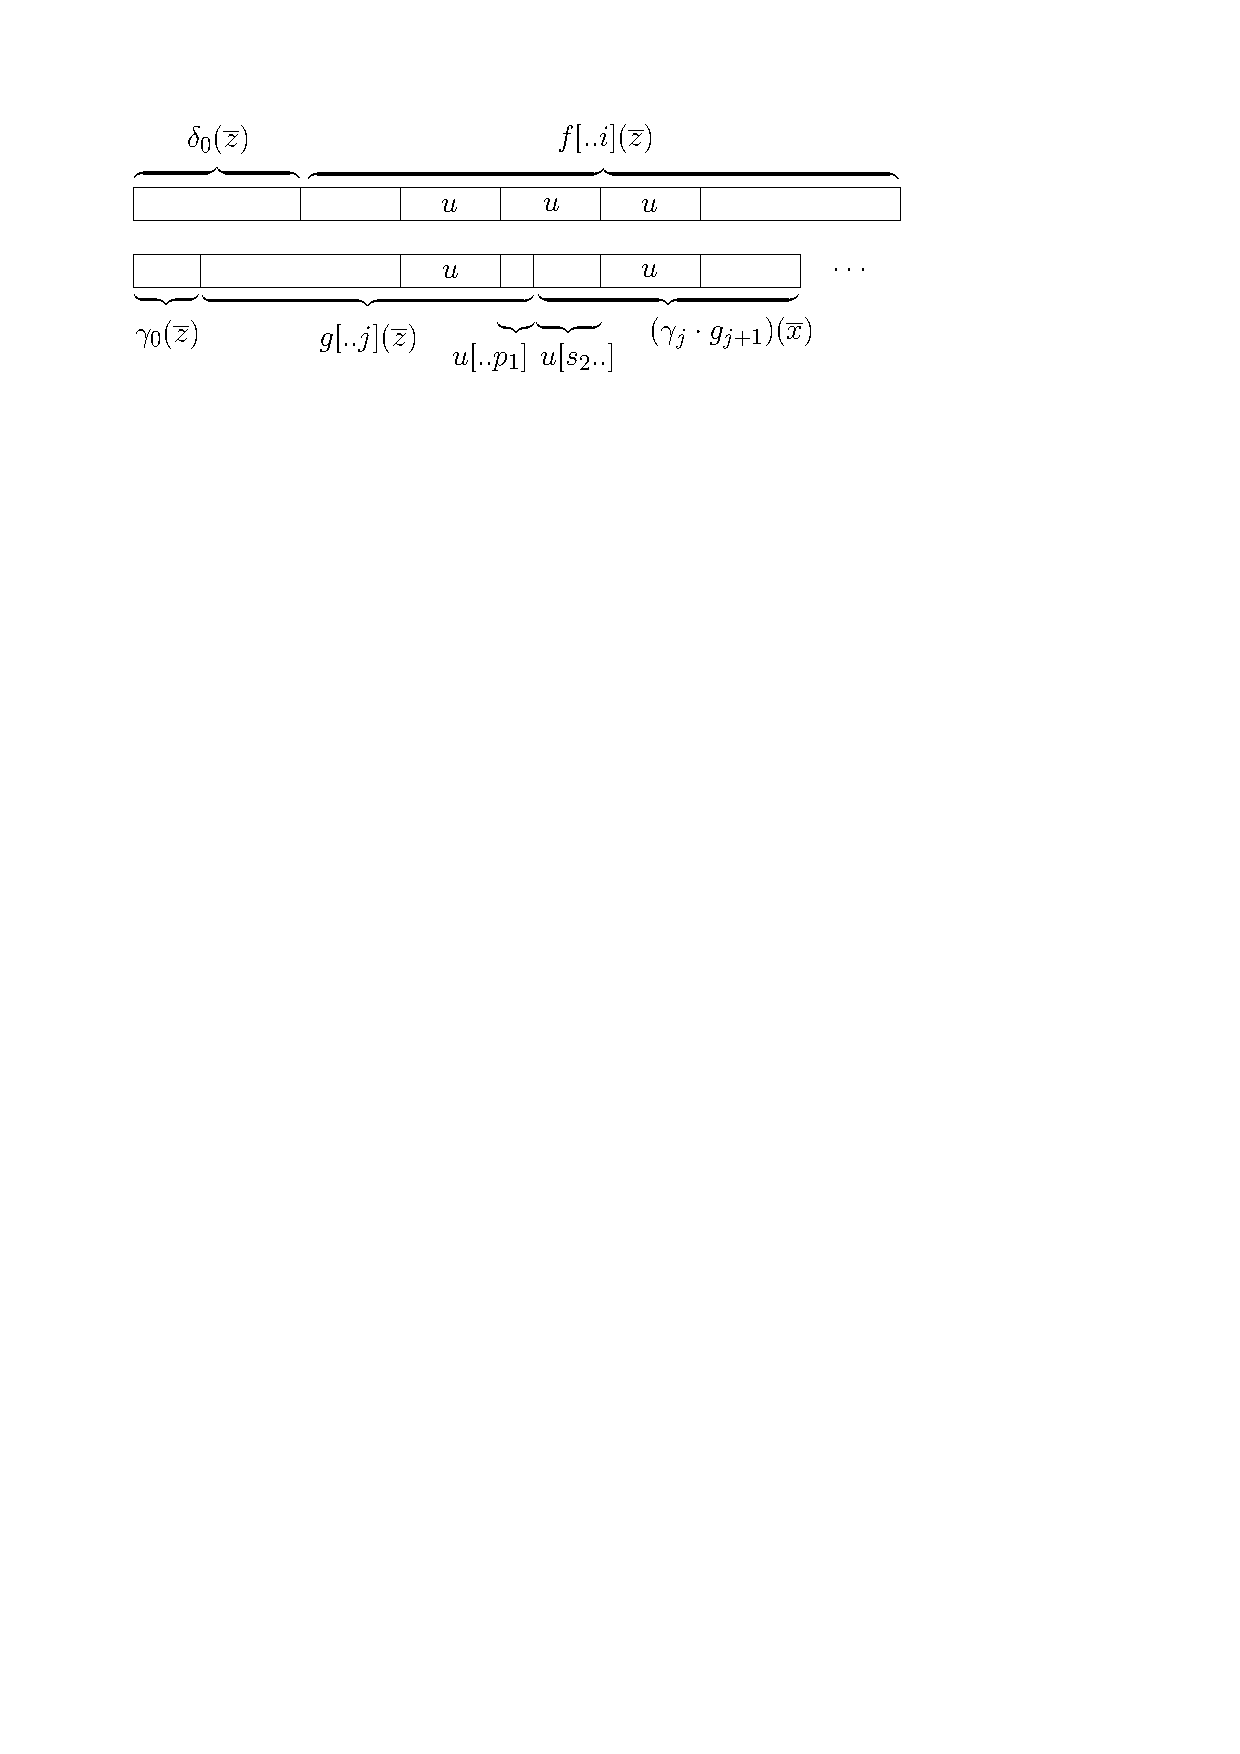
\includegraphics[width=0.8\linewidth]{pictures/bihoms_unary_extension.pdf}
        \caption{The choice of $\overline x$ and $\overline z$ ensures that the last occurence of $u$ in $\sfpref{g}{j}(\overline z)$ and the first occurence in $(\gamma_j \cdot g_{j+1})(\overline x)$ is covered exactly by some copies of $u$ in $\sfpref{f}{i}(\overline z)$. This implies that $\strpref{u}{p_1} \cdot \strsuf{u}{s_2} \in u^*$.}
        \label{fig:extending-the-unary-prefix}
    \end{figure}

    As commented above, this proves that mappings $p_2,s_1$ witness the fact that $\sfpref{g}{j+1}$ is $u$-unary, finishing the proof.
\end{proof}
\end{comment}
